% Kompilieren mit: TEXINPUTS=minted/source: pdflatex -shell-escape %
\documentclass[12pt,compress,ngerman,utf8,t]{beamer}
\usepackage[ngerman]{babel}
\usepackage{ragged2e}
\usepackage{comment}
\usepackage{minted}
\usepackage{wasysym}
\usepackage{tikz}
\usetikzlibrary{calc}
\usepackage[all]{xy}
\usepackage[protrusion=true,expansion=false]{microtype}

\hypersetup{colorlinks=true}

\title[Initiale Algebren]{\smiley{} Initiale Algebren \smiley}
\author[Augsburger Curry Club]{}
\date[2016-06-16]{}

\usetheme{Warsaw}

\useinnertheme{rectangles}

\usecolortheme{seahorse}
\definecolor{mypurple}{RGB}{150,0,255}
\setbeamercolor{structure}{fg=mypurple}
\definecolor{myred}{RGB}{150,0,0}
\setbeamercolor*{title}{bg=myred,fg=white}
\setbeamercolor*{titlelike}{bg=myred,fg=white}

\usefonttheme{serif}
\usepackage[T1]{fontenc}
\usepackage{libertine}

\newcommand{\slogan}[1]{%
  \begin{center}%
    \setlength{\fboxrule}{2pt}%
    \setlength{\fboxsep}{8pt}%
    {\usebeamercolor[fg]{item}\fbox{\usebeamercolor[fg]{normal text}\parbox{0.91\textwidth}{#1}}}%
  \end{center}%
}

\definecolor{darkred}{RGB}{220,0,0}
\newcommand{\hcancel}[5]{%
    \tikz[baseline=(tocancel.base)]{
        \node[inner sep=0pt,outer sep=0pt] (tocancel) {#1};
        \draw[darkred, line width=1mm] ($(tocancel.south west)+(#2,#3)$) -- ($(tocancel.north east)+(#4,#5)$);
    }%
}%

\renewcommand{\C}{\mathcal{C}}
\newcommand{\D}{\mathcal{D}}
\newcommand{\id}{\mathrm{id}}
\newcommand{\Id}{\mathrm{Id}}
\newcommand{\Hask}{\mathrm{Hask}}

\setbeamertemplate{navigation symbols}{}
\setbeamertemplate{headline}{}

\setbeamertemplate{title page}[default][colsep=-1bp,rounded=false,shadow=false]
\setbeamertemplate{frametitle}[default][colsep=-2bp,rounded=false,shadow=false,center]

\newcommand*\oldmacro{}%
\let\oldmacro\insertshorttitle%
\renewcommand*\insertshorttitle{%
  \oldmacro\hfill\insertframenumber\,/\,\inserttotalframenumber\hfill}

\newcommand{\hil}[1]{{\usebeamercolor[fg]{item}{\textbf{#1}}}}
\setbeamertemplate{frametitle}{%
  \vskip1em%
  \leavevmode%
  \begin{beamercolorbox}[dp=1ex,center]{}%
      \usebeamercolor[fg]{item}{\textbf{\textsf{\Large \insertframetitle}}}
  \end{beamercolorbox}%
}

\setbeamertemplate{footline}{%
  \leavevmode%
  \hfill%
  \begin{beamercolorbox}[ht=2.25ex,dp=1ex,right]{}%
    \usebeamerfont{date in head/foot}
    \insertframenumber\,/\,\inserttotalframenumber\hspace*{1ex}
  \end{beamercolorbox}%
  \vskip0pt%
}

\newcommand{\backupstart}{
  \newcounter{framenumberpreappendix}
  \setcounter{framenumberpreappendix}{\value{framenumber}}
}
\newcommand{\backupend}{
  \addtocounter{framenumberpreappendix}{-\value{framenumber}}
  \addtocounter{framenumber}{\value{framenumberpreappendix}}
}

\setbeameroption{show notes}
\setbeamertemplate{note page}[plain]

\begin{document}

% http://www.goodwp.com/images/201311/goodwp.com_30317.jpg
{\usebackgroundtemplate{
\includegraphics[height=\paperheight]{images/forest}}
\frame{\titlepage\vspace*{16em}}}

\frame{\tableofcontents}

\section{Motivation}

\begin{frame}\frametitle{Motivation}
  In der Mathematik und theoretischen Informatik untersucht man oft
  \hil{Fixpunktgleichungen}:
  \[ x = f(x) \]
  Oft ist man am \hil{kleinsten} oder \hil{größten} Fixpunkt interessiert:
  \[ \mu f \qquad\text{oder}\qquad \nu f \]

  \centering
  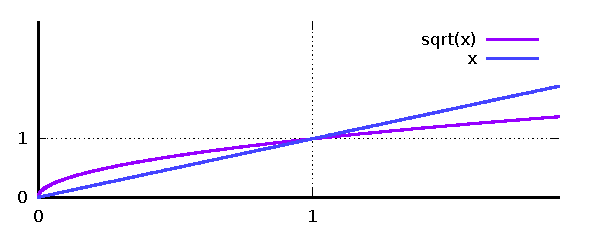
\includegraphics{fixpunkt}
  \par
\end{frame}

\begin{frame}[fragile]\frametitle{Motivation}
  In der theoretischen Informatik benötigt man aber auch
  eine höhere Art von Fixpunkt"`gleichungen"':
  \[ X \cong F(X) \]

  \hil{Initiale Algebren} verallgemeinern kleinste Fixpunkte,
  \hil{terminale Koalgebren} verallgemeinern größte Fixpunkte.
  \medskip

  Wir klären heute folgende Frage: Was bedeutet
  \begin{minted}{haskell}
             data Nat = Zero | Succ Nat
  \end{minted}
  eigentlich wirklich?
  \medskip

  Zunächst:
  "`keine Bottoms, alles endlich"'.
\end{frame}


\section{Algebren}

\subsection{Definition}

\begin{frame}[fragile]\frametitle{Algebren}
  Eine \hil{Algebra} für einen Funktor $F : \C \to \C$ besteht aus
  \begin{itemize}
    \item einem Objekt $A \in \C$ und
    \item einem Morphismus $\alpha : F(A) \to A$ in~$\C$.
  \end{itemize}

  \begin{minted}{haskell}
data F a = Nil | Cons Int a  -- Beispielfunktor

instance Functor F where
    fmap f Nil        = Nil
    fmap f (Cons x r) = Cons x (f r)

productA :: F Int -> Int  -- Beispielalgebra
productA Nil        = 1
productA (Cons x r) = x * r
  \end{minted}
\end{frame}

\begin{frame}[fragile]{Algebren sind nicht rar!}
  \begin{minted}{haskell}
data F a = Nil | Cons Int a

productA :: F Int -> Int
productA Nil        = 1
productA (Cons x r) = x * r

lengthA :: F Int -> Int
lengthA Nil        = 0
lengthA (Cons _ r) = 1 + r

allNonzeroA :: F Bool -> Bool
allNonzeroA Nil        = True
allNonzeroA (Cons x r) = x /= 0 && r
  \end{minted}
\end{frame}

\note{\justifying
  Eine Algebra für einen Funktor~$F$ kann man sich vorstellen wie die Anleitung
  für einen~$F$-förmigen Rekursionsschritt. Die Rekursion selbst wird aber
  nicht ausgeführt. Algebren machen Ideen, wie eine Rekursion zu führen sei,
  zu first-class values.
  \medskip

  Eine Algebra muss keinerlei Axiome erfüllen (anders als bei Monoiden, Gruppen
  oder Ringen). Das erklärt ihr universelles Vorkommen.
  \medskip

  Ist der verwendete Funktor~$F$ der zugrundeliegende Funktor einer Monade, so
  kann man Axiome an die Algebra stellen. Dann spricht man von "`Algebren
  für Monaden"'. In gewisser Hinsicht sind sie für die Mathematik, Logik und
  Informatik noch wichtiger als Algebren für Funktoren. Sie sind aber nicht
  Gegenstück dieses Vortrags.
  \par
}

\begin{frame}[fragile]{Ein besonderes Beispiel}
  \begin{minted}{haskell}
data F a = Nil | Cons Int a

productA :: F Int -> Int
productA Nil        = 1
productA (Cons x r) = x * r

allNonzeroA :: F Bool -> Bool
allNonzeroA Nil        = True
allNonzeroA (Cons x r) = x /= 0 && r

initialA :: F [Int] -> [Int]
initialA Nil        = []
initialA (Cons x r) = x : r
  \end{minted}
\end{frame}


\subsection{Morphismen zwischen Algebren}

\begin{frame}[fragile]{Morphismen zwischen Algebren}
  Ein \hil{Morphismus} zwischen~$F$-Algebren
  $\alpha : F(A) \to A$ und $\beta : F(B) \to B$ ist ein Morphismus
  $g : A \to B$
  sodass das folgende Diagramm kommutiert.
  \[ \xymatrixcolsep{3pc}\xymatrixrowsep{3pc}\xymatrix{
    F(A) \ar[r]^\alpha\ar[d]_{\operatorname{fmap} g} & A \ar[d]^g \\
    F(B) \ar[r]_\beta & B
  } \]

  \begin{minted}{haskell}
data F a = Nil | Cons Int a

g :: Int -> Bool
g x = x /= 0
-- g . productA = allNonzeroA . fmap g
  \end{minted}
\end{frame}


\subsection{Initiale Algebren}

\begin{frame}[fragile]{Initiale Algebren}
  Die "`besondere Beispielalgebra"' hat eine \hil{universelle Eigenschaft}:
  Sie ist die \hil{initiale} $F$-Algebra.

  \begin{minted}{haskell}
data F a = Nil | Cons Int a

initialA :: F [Int] -> [Int]
initialA Nil        = []
initialA (Cons x r) = x : r

cata :: (F a -> a) -> ([Int] -> a)
cata beta []     = beta Nil
cata beta (x:xs) = beta (Cons x (cata f xs))
-- cata beta . initialA = beta . fmap (cata beta)

product :: [Int] -> Int
product = cata productA
 \end{minted}
\end{frame}

\note{\justifying
  Eine~$F$-Algebra~$A$ heißt genau dann \emph{initial}, wenn es genau einen
  Algebrenmorphismus~$A \to B$ in jede~$F$-Algebra~$B$ gibt.
  \medskip

  Ist~\texttt{beta :: F a -> a} eine solche beliebige~\texttt{F}-Algebra, so
  ist~\texttt{cata beta :: [Int] -> a} dieser eindeutige Morphismus.
  \par
}

\note{\justifying
  Viele (aber nicht alle) Datentypen "`von endlichen Dingen"' in Haskell
  sind Beispiele für initiale Algebren:

  \inputminted{haskell}{images/initial-algebras.hs}

  Entsprechend sind viele (struturell-)rekursive Funktionen Beispiele für
  Katamorphismen -- also Morphismen, die uns die universelle Eigenschaft der
  initialen Algebren schenken.
  \par
}

\begin{frame}[fragile]{Gibt es immer initiale Algebren?}
  Sei~$F : \C \to \C$ ein Funktor. Gibt es eine initiale~$F$-Algebra?
  \pause
  Antwort: \hil{Manchmal} (hängt von~$\C$ und~$F$ ab). Aber in
  der Kategorie der Haskell-Typen und Haskell-Funktionen immer (zumindest
  moralisch), denn man kann sie explizit konstruieren:
  \medskip

  \begin{minted}{haskell}
data Mu f = MkMu { outF :: f (Mu f) }
-- mit sozialer Vereinbarung, nur "endliche" Werte zu
-- betrachten. Der Morphismenanteil der initialen
-- Algebra ist MkMu :: f (Mu f) -> Mu f.

cata :: (Functor f) => (f a -> a) -> (Mu f -> a)
cata g (MkMu r) = g (fmap (cata g r))
  \end{minted}
  \pause

  \slogan{Initiale Algebren modellieren Datentypen, für die man Funktionen
  heraus durch Rekursion angeben kann.}
\end{frame}

\note{\justifying
  Kategorielles Fun Fact: Ist eine Kategorie sowohl vollständig (besitzt für
  jedes kleine Diagramm eines Limes) als auch "`algebraisch vollständig"'
  (besitzt für jeden Endofunktor eine initiale Algebra), so ist sie schon dünn
  (je zwei parallele Morphismen sind gleich), kommt also von einer Quasiordnung
  her.
  \medskip

  Das ist ein
  \href{https://cstheory.stackexchange.com/questions/21028/algebraically-compact-categories}{Theorem
  von Freyd}.
  \par
}

\begin{frame}{Endlichkeit}
  Initiale Algebren modellieren Datentypen, für die jeder Wert "`endlich"' ist.
  \medskip

  Tatsächlich kann man in vielen Kategorien die initale Algebra eines
  Funktors~$F$ gewinnen als
  \[ \mu F = \operatorname{colim}(\emptyset \to F(\emptyset) \to F(F(\emptyset)) \to \cdots). \]
  Dabei ist~$\emptyset$ das initiale Objekt (der leere Datentyp~\texttt{Void}).
\end{frame}

\note{\justifying
  Ist~$F$ der Funktor der vorherigen Folien, so realisiert die gezeigte Formel
  für~$\mu F$ als (Ko-)Limes der Datentypen der leeren Listen, der höchstens
  einelementigen Listen, der höchstens zweielementigen Listen, und so
  weiter.\par
}


\subsection{Lambeks Lemma}

\begin{frame}{Lambeks Lemma}
  Sei~$\alpha : F(A) \to A$ eine initiale Algebra.
  Dann ist~$\alpha$ ein Isomorphismus (besitzt einen Umkehrmorphismus).
  \medskip

  In diesem Sinn löst~$A$ die Fixpunkt"`gleichung"'
  \[ X \cong F(X). \]
  Anschaulich: Mit~$\alpha$ konstruiert man neue Werte aus alten. \\
  Die Isomorphie bedeutet, dass jeder Wert aus anderen Werten konstruierbar ist.
  \bigskip
  \pause

  \centering
  \hil{Übungsaufgabe!} \\
  Wie viele Hilfsmorphismen benötigst du?
  \par
\end{frame}

\note{\justifying
  Eine Art Umkehrung von Lambeks Lemma gilt nicht: Ist der
  Strukturmorphismus~$F(A) \to A$ einer Algebra zufälligerweise ein
  Isomorphismus, so heißt das noch nicht, dass sie eine initiale Algebra ist.
  \medskip

  Ist die Basiskategorie~$\C$ nämlich eine Partialordnung, so sind initiale
  Algebren dasselbe wie kleinste Fixpunkte und terminale Koalgebren dasselbe
  wie größte Fixpunkte. Aber nicht jeder Fixpunkt ist ein kleinster.
  \par
}


\section{Terminale Koalgebren}

\begin{frame}[fragile]{Terminale Koalgebren}
  Eine \hil{Algebra} für einen Funktor $F : \C \to \C$ besteht aus
  \begin{itemize}
    \item einem Objekt $A \in \C$ und
    \item einem Morphismus $\alpha : F(A) \to A$ in~$\C$.
  \end{itemize}
  \medskip

  Eine \hil{Koalgebra} für einen Funktor $F : \C \to \C$ besteht aus
  \begin{itemize}
    \item einem Objekt $A \in \C$ und
    \item einem Morphismus $\alpha : A \to F(A)$ in~$\C$.
  \end{itemize}
  \medskip

  \begin{minted}{haskell}
data Nu f = MkNu { outF :: f (Nu f) }
-- ohne sozialen Vertrag!

ana :: (Functor f) => (a -> f a) -> (a -> Nu f)
ana alpha x = MkNu (fmap (ana alpha) (alpha x))
  \end{minted}
\end{frame}

\note{\justifying
  Eine Koalgebra für einen Funktor~$F$ kann man sich vorstellen wie die Anleitung
  für eine~$F$-förmige Beobachtung. Die Beobachtung wird aber nicht "`bis zum
  Ende"', verschachtelt, korekursiv ausgeführt, sondern nur für einen Schritt
  lang. Koalgebren machen also Ideen, wie eine Korekursion zu führen sei, zu
  first-class values.
  \medskip

  Eine \emph{terminale Koalgebra} ist eine Koalgebra~$\beta : A \to F(A)$,
  sodass für jede Koalgebra~$\alpha : Z \to F(Z)$ genau ein Morphismus~$g : Z
  \to A$ mit $\beta \circ g = \operatorname{fmap} g \circ \alpha$ existiert.
  \[ \xymatrixcolsep{3pc}\xymatrixrowsep{3pc}\xymatrix{
    Z \ar[r]^\alpha\ar[d]_{g} & F(Z) \ar[d]^{\operatorname{fmap} g} \\
    A \ar[r]_\beta & F(A)
  } \]
}

\note{\justifying
  Wir haben bereits gesehen, dass viele Datentypen "`von endlichen Dingen"' in
  Haskell initiale Algebren sind. Viele Datentypen "`von nicht notwendigerweise
  endlichen Dingen"' sind terminale Koalgebren:

  \inputminted{haskell}{images/terminal-coalgebras.hs}

  Entsprechend sind viele (strukturell-)korekursive Funktionen Beispiele für
  Anamorphismen -- also Morphismen, die uns die universellen Eigenschaften
  terminaler Koalgebren schenken.
  \par
}

\note{\justifying
  Übungsaufgabe: Wieso spricht niemand über terminale Algebren und initiale
  Koalgebren?
  \par
}


\section{Vergleich}

\begin{frame}[fragile]{Vergleich}
  Initiale Algebren modellieren Datentypen, für die man Funktionen
  heraus durch Rekursion angeben kann.

  \begin{itemize}
    \item Konstruktion von Werten mittels $F(A) \to A$
    \item \mintinline{haskell}{cata :: (F a -> a) -> (Mu F -> a)}
    \item "`endlich"'
  \end{itemize}

  \bigskip

  Terminale Koalgebren modellieren Datentypen, für die man Funktionen
  hinein durch Korekursion angeben kann.

  \begin{itemize}
    \item Beobachtung von Werten mittels $A \to F(A)$
    \item \mintinline{haskell}{ana :: (a -> F a) -> (a -> Nu F)}
    \item "`endlich oder unendlich"'
  \end{itemize}
\end{frame}

\note{\justifying
  Das Wesentliche an einer initialen Algebra~$A$ ist, dass man vermöge der
  mitgegebenen Funktion~$F(A) \to A$ Werte von~$A$ \emph{konstruieren} kann.
  Wir stellen uns~$F(A)$ als den Datentyp der Konstruktionsbeschreibungen für
  Werte von~$A$ vor; die Funktion~$F(A) \to A$ nimmt eine solche Beschreibung
  und führt sie aus.
  \medskip

  \emph{Beispiel:} \texttt{initialA (Cons x xs)} konstruiert die verlängerte
  Liste \texttt{x:xs}.
  \medskip

  Das Wesentliche an einer terminalen Koalgebra~$A$ ist, dass man vermöge der
  mitgegebenen Funktion~$A \to F(A)$ Werte von~$A$ \emph{beobachten} kann.
  Wir stellen uns~$F(A)$ als den Datentyp der möglichen Beobachtungen über
  Werte von~$A$ vor.
  \medskip

  \emph{Beispiel:} \texttt{terminalCoA xs} beobachtet, ob die übergebene
  Liste~\texttt{xs} leer ist oder eine Cons-Zelle ist (aus einem vorderen
  Element~\texttt{x} und einer Restliste~\texttt{xs'} besteht).
  \par
}

\note{\justifying
  Lambeks Lemma garantiert, dass die zu einer initialen Algebra gehörige
  Funktion~$F(A) \to A$ (bzw. die zu einer terminalen Koalgebra gehörige
  Funktion~$A \to F(A)$) umkehrbar ist. Daher kann man aus einer initialen
  Algebra eine Koalgebra (welche nur in pathologischen Fällen terminal
  sein wird) und dual aus einer terminalen Koalgebra eine Algebra machen.
  \medskip

  \emph{Beispiel:} Das Wesentliche vom Datentyp der endlichen Listen ist, dass
  man seine Werte aus Grundbestandteilen (\texttt{Nil} und \texttt{Cons x})
  sukzessive \emph{konstruieren} kann. Trotzdem kann man seine Werte auch \emph{beobachten}
  (prüfen, ob ein Wert \texttt{Nil} ist oder eine Cons-Zelle ist).
  \medskip

  \emph{Beispiel:} Das Wesentliche vom Datentyp der nicht notwendigerweise
  endlichen Listen ist, dass man seine Werte \emph{beobachten} kann (ist eine solche
  Liste leer oder eine Cons-Zelle?). Trotzdem kann man aber auch seine Werte
  \emph{konstruieren} (etwa an eine gegebene beliebig lange Liste vorne ein Element
  anfügen).
  \par
}


\section{Ausblick}

% http://memory-alpha.wikia.com/wiki/Where_No_Man_Has_Gone_Before_(episode)
\usebackgroundtemplate{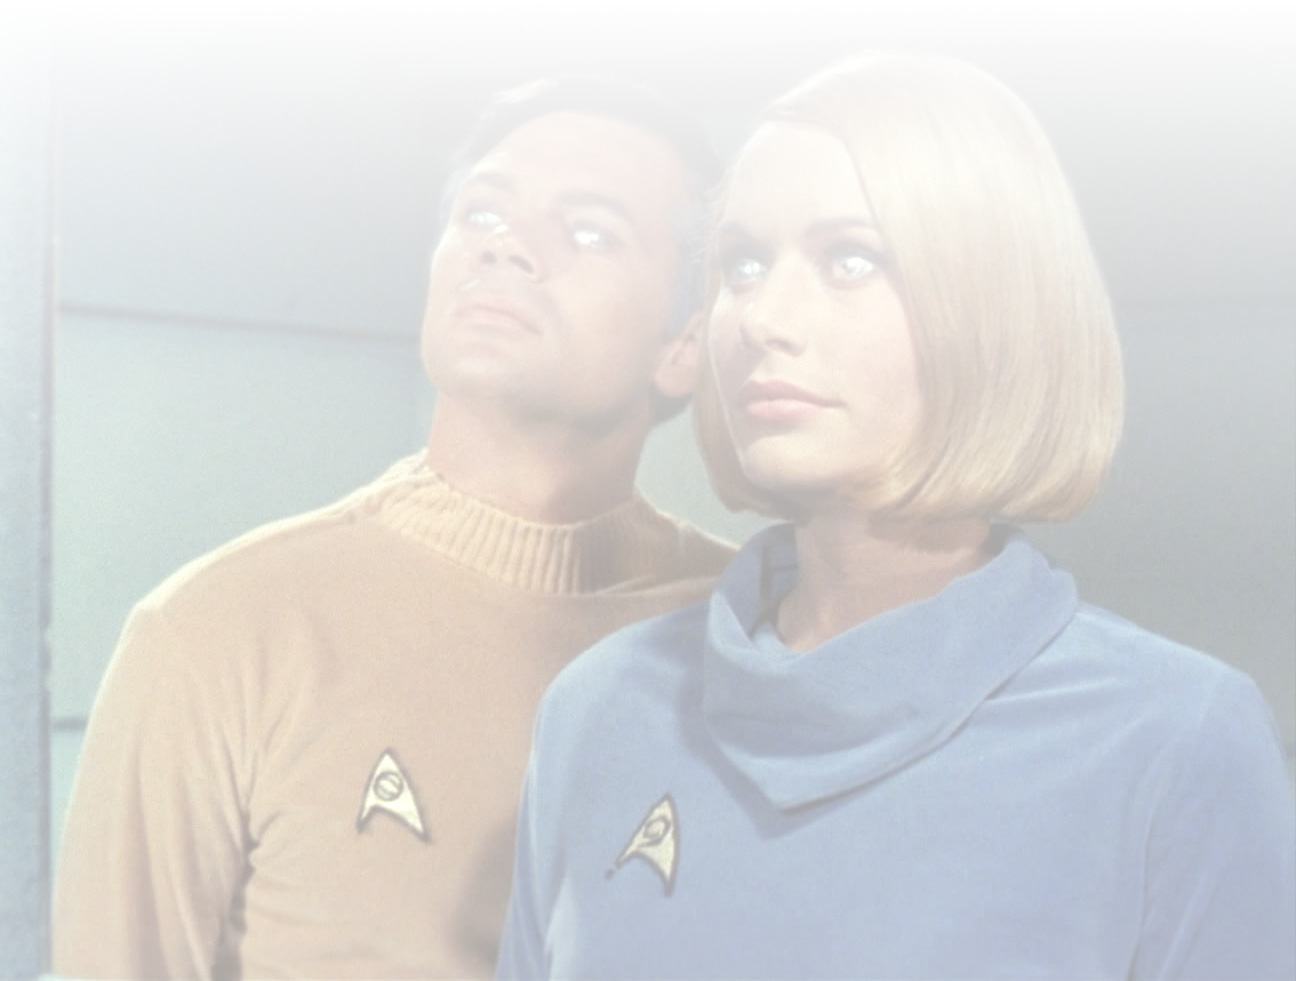
\includegraphics[width=\paperwidth]{images/where-no-man-has-gone-before}}
\begin{frame}[fragile]{Ausblick}
  \begin{itemize}
    \item Behandlung von Bottoms durch Wechsel der Kategorie --
    nicht die Kategorie der Mengen, sondern die Kategorie der \hil{Domänen}
    (domains)
    \pause

    \item Haskell: boldly going where no functor has gone before.

    \begin{minted}{haskell}
data Seltsam = MkSeltsam (Seltsam -> Bool)
    \end{minted}
  \end{itemize}
\end{frame}

\note{\justifying
  Die Theorie der initialen Algebren und terminalen Koalgebren ist nur der
  Anfang. Für Datentypen, die durch eine kompliziertere Rekursionsgleichung
  gegeben sind (etwa, wo der verwendete Funktor kontra- statt kovariant ist; wo
  der verwendete Funktor in einem Argument ko- und in einem anderen
  kontravariant ist; wo es gar keinen erkennbaren Funktor mehr gibt), benötigt
  man eine leistungsfähigere Theorie.
  \medskip

  Die Kategorie der Domänen hat sich als sehr leistungsfähig erwiesen. In ihr
  gibt es viel mehr als nur initiale Algebren und terminale Koalgebren.
  \par
}

\note{\justifying
  Mehr zum seltsamen Typ hat
  \href{http://blog.sigfpe.com/2008/01/type-that-should-not-be.html}{Dan Piponi
  zu berichten}. Der Typ ist durchaus beachtenswert, liefert er doch ein
  Gegenbeispiel zu einer (internen Variante von) Cantors Theorem:
  \medskip

  In früheren Curry-Club-Vorträgen haben wir gesehen, dass keine Menge~$X$
  isomorph zu ihrer Potenzmenge~$\mathcal{P}(X)$ sein kann. ("`Isomorph"' heißt
  hier "`gleich mächtig"' und die Potenzmenge ist die Menge aller Teilmengen
  von~$X$, verallgemeinerbarer formuliert als Menge aller Abbildungen von~$X$
  nach~Bool.)
  \medskip

  Eine Domäne~$X$ kann aber durchaus isomorph zu ihrer "`Potenzdomäne"'~$(X \to
  \mathrm{Bool})$ sein. Das ist etwa bei \texttt{Seltsam} der Fall.
  \par
}

\end{document}
